\subsection{Estructura de l'aplicació}
\label{sec:etapa1}

L'estructura de l'aplicació és la primera etapa, i prerequisit de la resta d'etapes. L'objectiu és el d'obtenir un esquelet base d'aplicació iOS per a poder implementar les funcionalitats que es demanen.
Aquesta base ha de tenir les següents funcionalitats:

\begin{compactitem}
    \item El sistema ha de demanar a l'usuari que introdueixi les seves credencials.
    \item Les dades que ha introduït l'usuari s'han de validar amb el servei d'autenticació.
    \item Si les dades són correctes s'ha d'obtenir el \textit{token} de l'usuari, si no són correctes s'ha d'informar a l'usuari del problema.
    \item El sistema ha d'establir la connexió amb el MAX amb el \textit{token} de l'usuari.
    \item El sistema ha de poder obtenir informació d'algun dels serveis del MAX, com per exemple el \textit{timeline}.
\end{compactitem}

Aquesta etapa inclou les històries d'usuari 1 i 2 (pàgina \pageref{sec:historia_1}).

\subsubsection{Implementació}
A l'iniciar aquesta etapa es partia de zero ja que era l'inici del projecte. Abans de començar a crear el projecte es va fer un petit estudi de la situació, per poder decidir quina estructura era la millor i com fer la connexió al MAX.

L'estructura de la interfície està fixa pel client que va demana que l'aplicació estigui estructura en pestanyes, i dintre de les pestanyes s'ha de navegar utilitzant la barra de navegació. 

Sobre l'estructura interna de l'aplicació es va decidir seguir els patrons habituals de disseny que proposa \textit{Apple}\cite{apple_disseny}. Aquests patrons en essència són:

\begin{itemize}
    \item \textit{Model-View-Controller} (Model-Vista-Controlador, MVC) \footnote{\url{https://developer.apple.com/library/ios/documentation/General/Conceptual/DevPedia-CocoaCore/MVC.html}}: Aquest patró de disseny s'utilitza per a estructurar tota l'aplicació.
    \item \textit{Delegation} (Delegació) \footnote{\url{https://developer.apple.com/library/ios/documentation/General/Conceptual/DevPedia-CocoaCore/Delegation.html}}: Facilita la transmissió d'informació i dades d'un objecte a un altre.
    \item \textit{Target-action} \footnote{\url{https://developer.apple.com/library/ios/documentation/General/Conceptual/Devpedia-CocoaApp/TargetAction.html}}: Patró de disseny que relaciona les interaccions de l'usuari (botons i controls) amb el codi que la aplicació ha d'executar.
    \item \textit{Block objects} \footnote{\url{https://developer.apple.com/library/ios/documentation/General/Conceptual/DevPedia-CocoaCore/Block.html}}: Utilitza blocs de codi per implementar \textit{callbacks} i codi asíncron.
\end{itemize}

Un dels punts més importants va ser prendre una decisió sobre com connectar el sistema amb el MAX. Per fer-ho es van considerar tres possibilitats:
\begin{itemize}
    \item  \textbf{Fer les crides des de l'aplicació}: consisteix en realitzar totes les consultes i modificacions des de l'aplicació i d'aquesta manera fer tot el sistema molt eficient. Aquesta solució té l'inconvenient de presentar un alt nivell d'acoblament entre l'aplicació i el MAX, i per tant, el codi resultant seria molt poc canviable.
    \item  \textbf{Implementar una llibreria}: aquesta possibilitat implica desenvolupar una llibreria externa a l'aplicació que permeti obtenir la informació del MAX mitjançant una API en Objective-C. Aquesta solució ofereix un bon nivell de canviabilitat ja que els canvis en el MAX només comportarien canvis a la llibreria. Aquesta opció implica un gran esforç de desenvolupament.
    \item  \textbf{Utilitzar una llibreria que facilit la connexió}: en aquest cas s'hauria de fer una cerca de possibles llibreries i posteriorment triar la més adient per a aquest cas. L'objectiu és delegar a la llibreria desenvolupada per un tercer la responsabilitat d'establir i mantenir la connexió amb el MAX, així com fer totes les consultes i modificacions seguint la filosofia REST. El principal inconvenient d'aquesta opció és el de limitar el desenvolupament a les funcionalitats que ofereix la llibreria.
\end{itemize}

Es va decidir descartar la primera opció ja que el producte resultant seria difícil de mantenir. Per decidir entre la segona i la tercera opció es va fer una petita cerca de llibreries de tercers.

Com a resultat de la cerca es van obtenir quatre llibreries que cumplien amb els requisits:
\begin{itemize}
    \item  ASIHTTPRequest \footnote{\url{http://allseeing-i.com/ASIHTTPRequest/}}: aquesta llibreria facilita l'establiment de connexions amb el servidor per a fer consultes oferint una API de més alt nivell que les consultes natives d'Objective-C. El problema principal d'aquesta llibreria és que no té un suport continuat ni s'adapta a les necessitats del projecte.
    \item  AFNetworking \footnote{\url{https://github.com/AFNetworking/AFNetworking}}: llibreria similar a ASIHTTPRequest, facilita l'establiment de connexions amb una API de més alt nivell que la nativa. De la mateixa manera que amb l'anterior llibreria, aquesta no és la més adient per al projecte ja que només facilita l'accés al servidor, però no facilita la implementació dels principis REST.
    \item  RestKit \footnote{\url{https://github.com/RestKit/RestKit}}: aquesta llibreria proporciona una interficie completa per a que l'aplicació es comuniqui amb un servidor REST de forma semi-transparent. És a dir que l'aplicació ha de configurar tots els mapeigs dels serveis del servidor i posteriorment l'aplicació només ha de fer les crides a RestKit, que les transformarà en crides REST.
    \item  Spaghetti \footnote{\url{https://github.com/noodlewerk/Spaghetti}}: llibreria similar a RestKit però per servidors que no utilitzen el protocol REST, per tant aquesta llibreria és més flexible que la anterior.
\end{itemize}

Després d'estudiar i analitzar totes les possibilitats es va decidir fer una prova de concepte amb la llibreria RestKit\cite{restkit}. Perquè era la que més s'ajustava a les necessitats del projecte i podia aportar més valor. 

La prova de concepte va consistir en crear el projecte de l'aplicació. Es va partir d'una plantilla d'aplicació amb pestanyes que ofereix \textit{Apple}. Es va afegir la llibreria RestKit i es va provar de configurar amb un \textit{token} del MAX posat manualment. El primer servei que es va intentar utilitzar va ser el del \textit{timeline}. Es va configurar el mapeig del servei i el mapeig del model de dades (seguint l'estàndard ActivityStream\cite{activityStream}).

Una vegada obtingudes amb èxit les dades del MAX del \textit{timeline} mitjançant la prova de concepte, es va decidir utilitzar RestKit per al projecte.

A partir d'aquí es va continuar amb el desenvolupament afegint la pantalla d'inici de sessió. Per a validar l'usuari no es va utilitzar RestKit, si no que es va fer una consulta directament amb el servei de validació de la UPC ja que aquest no funciona amb REST si no que segueix el protocol d'\textit{OAuth2}\cite{oauth2}. A la figura \ref{fig:limit_restkit} es pot veure a quins àmbits s'utilitza RestKit i a quins no s'utilitza.

\begin{figure}[ht]
    \centering
    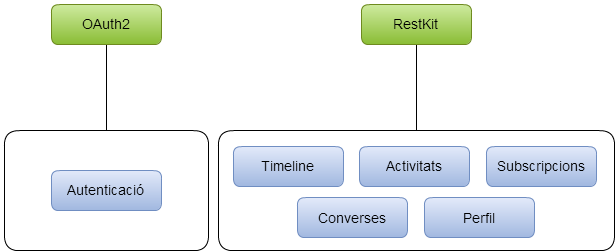
\includegraphics[scale=0.6]{Memoria/Implementacio/LimitRestKit.png}
    \caption{Limit d'ús de la llibreria RestKit.}
    \label{fig:limit_restkit}
\end{figure}


Un cop l'usuari estava validat s'obtenia el \textit{token} i ja es podia configurar RestKit amb el nom d'usuari i el \textit{token} de l'usuari que havia iniciat sessió.




